% !TEX root = ../Thesis.tex

\chapter{Gestione della memoria in Rust}\label{cap:03}

In questo capitolo viene esaminato l'approccio implementato da Rust per gestire la memoria dinamica. In particolare, verranno approfonditi concetti chiave come \textit{Ownership}, \textit{Borrowing} e \textit{Lifetime}, illustrandone il funzionamento. L'obiettivo è evidenziare come Rust possa garantire la sicurezza della memoria senza sacrificare le prestazioni.

Le informazioni presentate in questo capitolo sono tratte principalmente dalla documentazione ufficiale di Rust~\cite{rust-book}. \hfill
\vspace{15pt}
\noindent L'approccio implementato da Rust per gestire la memoria dinamica è noto come `modello di ownership' (\textit{Ownership Model}). Il modello si fonda sui concetti di \textit{ownership}, \textit{borrowing} e \textit{lifetime}, i quali stabiliscono regole sulla gestione della memoria che devono essere rispettate affinché il codice sia compilabile. Il rispetto di tali regole costituisce un prerequisito per la compilazione. Il compilatore controlla che ogni vincolo sia soddisfatto e procede alla compilazione solo in caso positivo. Il modello garantisce un uso corretto e sicuro della memoria già a tempo di compilazione, evitando l'introduzione di overhead durante l'esecuzione\footnote{È opportuno precisare che un minimo overhead viene comunque introdotto, sotto forma di invocazione  automatica di una funzione dedicata alla deallocazione.}.
\section{Ownership}
Il primo concetto alla base del modello di ownership di Rust è l'\textit{ownership}\footnote{Sebbene innovativo, questo concetto non è unico di Rust, il quale ha infatti preso spunto da un pattern ampiamente utilizzato in C++: \textit{RAII} (Resource Allocation Is Initialization), secondo il quale gli oggetti acquisiscono le risorse di cui hanno bisogno (ovvero vengono inizializzati) al momento della loro allocazione.} stessa, la quale definisce vincoli sui legami tra variabili e valori. Rust introduce il concetto di \textit{proprietario}: ogni valore ha un proprietario, ovvero la variabile che lo possiede in un determinato istante.

Si consideri, come esempio, la seguente assegnazione: \texttt{a = 5}.
Nella maggior parte dei linguaggi di programmazione, l'istruzione verrebbe interpretata come `\textit{a vale 5}'. In Rust il significato è diverso: `\textit{a possiede il valore 5}' o `\textit{a è il proprietario di 5}'. \\
\indent Stabilire i proprietari è fondamentale per implementare un meccanismo di deallocazione della memoria deterministico e prevedibile: chi libera la memoria relativa a un determinato valore? Il suo proprietario. \hfill
\vspace{5pt}\\
\noindent Le regole di \textit{ownership}, quindi, stabiliscono i vincoli sui legami tra valori e proprietari. Esse sono tre:
\begin{itemize}
    \item Ogni valore ha un proprietario (owner);
    \item Può esserci un solo proprietario per volta (per ogni valore);
    \item Quando il proprietario di un valore esce dallo scope\footnote{Lo scope rappresenta un range nel programma all'interno del quale un oggetto è valido. Solitamente è delimitato da una coppia di parentesi graffe.}, il relativo valore viene scartato.
\end{itemize}

\noindent In Rust la memoria viene liberata automaticamente quando il proprietario di un valore esce dallo scope. Per implementare questo, Rust invoca una funzione speciale, \textit{drop}, in corrispondenza della fine di ogni scope. La funzione viene invocata su ogni variabile che esce dallo scope ed è il proprietario di un valore.

Grazie alle regole di \textit{ownership}, Rust può garantire che la deallocazione della memoria avvenga sempre in modo corretto: poiché ogni valore ha un solo proprietario, non vi è ambiguità riguardo a chi sia responsabile della sua deallocazione. Valgono le seguenti due proprietà:
\begin{itemize}
    \item L'esistenza di un proprietario garantisce che non vi siano valori allocati ma non più referenziati;
    \item L'unicità del proprietario impedisce che un'area di memoria venga deallocata più volte.
\end{itemize}

\noindent Le regole di \textit{ownership} influenzano diversi aspetti del linguaggio, in particolare la condivisione dei valori tra variabili, l'assegnazione, il passaggio di parametri alle funzioni e operazioni analoghe.

Per comprendere a fondo il comportamento del modello di \textit{ownership}, è utile esaminare come Rust gestisce i diversi tipi di dato. I tipi di dato si distinguono tra \textit{semplici} e \textit{complessi}:
\begin{itemize}
    \item I tipi semplici hanno dimensione fissa, nota a tempo di compilazione, e vengono quindi allocati nello stack;
    \item I tipi complessi, invece, hanno dimensione variabile o non determinabile a tempo di compilazione e vengono quindi allocati nell'heap.
\end{itemize}
In relazione alla gestione della memoria, Rust definisce due comportamenti distinti per l'assegnazione:
\begin{itemize}
    \item \textit{Copy}: l'intera memoria del valore viene duplicata tramite una copia bitwise; questo comportamento è adottato di default per i tipi semplici;
    \item \textit{Move}: il valore viene trasferito da una variabile all'altra, invalidando quella di origine; questo comportamento è adottato di default per i tipi complessi.
\end{itemize}

\noindent I frammenti di codice nei Listati~\ref{ownership:copy-example} e~\ref{ownership:move-example} illustrano il comportamento dell'assegnamento nei tipi semplici, che implementano \texttt{Copy}, e in quelli complessi, che implementano \texttt{Move}:
\begin{lstlisting}[language=Rust, caption={Comportamento di Copy}, label={ownership:copy-example}]
fn main() {
    let x: i32 = 5;
    let y: i32 = x;
    println!("x: {}, y: {}", x, y);
}
\end{lstlisting}
\begin{lstlisting}[language=Rust, caption={Comportamento di Move}, label={ownership:move-example}]
fn main() {
    let x: String = String::from("Sono in Heap!");
    let y: String = x;
    println!("x: {}, y: {}", x, y); // <-- Errore di compilazione
}
\end{lstlisting}
Nel Listato~\ref{ownership:copy-example} si osserva che \texttt{x} resta valido dopo l'assegnamento, poiché \texttt{i32} implementa \texttt{Copy}, trattandosi di un tipo semplice, allocato nello stack.

Nel Listato~\ref{ownership:move-example}, invece, l'assegnamento provoca il trasferimento dell'ownership, che viene trasferita a \texttt{y}, invalidando \texttt{x}. \texttt{String} è infatti un tipo complesso, allocato nell'heap, che non implementa \texttt{Copy} ma utilizza il comportamento di \texttt{Move} per impostazione predefinita. \hfill
\vspace{10pt}\\
\noindent Come visto nel Listato~\ref{ownership:move-example}, l'assegnamento di un tipo complesso trasferisce l'\textit{ownership}, rendendo invalido il riferimento originale. Questo comportamento, tuttavia, può risultare limitante in alcuni scenari.

Per ovviare a tale limitazione, Rust fornisce un meccanismo per effettuare copie profonde anche con tipi che utilizzano \texttt{Move}: il comportamento \texttt{Clone}\footnote{La clonazione può introdurre costi in temini di prestazioni, in quanto richiede operazioni di lettura e scrittura nella memoria Heap.}.

\texttt{Clone} permette di definire esplicitamente come realizzare la copia profonda di un valore. L'invocazione del metodo \texttt{clone()} genera un nuovo valore, indipendente dal primo, ma con lo stesso contenuto.

Si consideri l'esempio nel Listato~\ref{ownership:clone-example}, che mostra il comportamento di \texttt{Clone}:\hfill
\begin{lstlisting}[language=Rust, caption={Comportamento di Clone}, label={ownership:clone-example}]
fn main() {
    let x: String = String::from("Sono in Heap!");
    let y: String = x.clone();
    println!("x: {}, y: {}", x, y); // Entrambi i riferimenti sono validi
}
\end{lstlisting}
Nel Listato~\ref{ownership:clone-example} si osserva che sia \texttt{x} che \texttt{y} sono validi in seguito all'assegnamento, in quanto la chiamata a \texttt{clone()} ha generato una nuova stringa, con lo stesso contenuto, ma indipendente dalla prima. \hfill
\vspace{10pt}\\
\noindent Un'ulteriore limitazione del meccanismo di \textit{ownership} si presenta durante l'invocazione di una funzione, in particolare, nel passaggio di un valore come parametro.
Rust gestisce il passaggio di un parametro a una funzione in maniera analoga agli assegnamenti: le stesse regole di \texttt{Copy} e \texttt{Move} continuano ad applicarsi.

Si consideri l'esempio nel Listato~\ref{ownership:func-example} che illustra il comportamento di Rust nel passaggio a funzione di un valore di tipo semplice e di uno di tipo complesso:
\begin{lstlisting}[language=Rust, caption={Trasferimento di ownership nelle chiamate a funzione}, label={ownership:func-example}]
fn my_func(first: i32, second: String) {
    println!("Parametro 'first' {}", first);
    println!("Parametro 'second' {}", second);
}

fn main() {
    let x: i32 = 5;
    let y: String = String::from("move!");
    my_func(x, y);
    println!("Variabile originale x: {}", x); // <-- Ok
    println!("Variabile originale y: {}", y); // <-- Errore di compilazione: ownership trasferita
}
\end{lstlisting}
Nel Listato~\ref{ownership:func-example} si osserva che, passando un valore di tipo semplice come \texttt{x} (che implementa \texttt{Copy}), la variabile rimane valida anche dopo la chiamata alla funzione. Al contrario, passando \texttt{y}, di tipo \texttt{String} (che implementa \texttt{Move}), l'\textit{ownership} viene trasferita al parametro \texttt{second}. Terminata l'esecuzione di \texttt{my\_func}, \texttt{second} esce dallo scope e il valore viene deallocato, rendendo \texttt{y} una variabile non più valida.

Tale comportamento può risultare limitante in molte situazioni pratiche, dove si desidera utilizzare un valore senza trasferirne la proprietà. Per risolvere questo problema, Rust introduce un secondo meccanismo fondamentale: il \textit{borrowing}.

\section{Borrowing}
Dopo l'\textit{ownership}, il secondo concetto fondamentale su cui si fonda il modello di gestione della memoria di Rust è il \textit{borrowing}. Questo meccanismo consente la condivisione sicura dei dati, permettendo di accedere temporaneamente a un valore senza acquisirne la proprietà.

Rust implementa concretamente il \textit{borrowing} tramite il concetto di \textit{reference}. Una \textit{reference} può essere vista come un puntatore: rappresenta un indirizzo che può essere seguito per accedere al valore memorizzato a tale indirizzo; tale valore appartiene a un'altra variabile.
\break  \break
\noindent In generale, le variabili in Rust, sia di tipo primitivo che reference, sono immutabili per default: non possono essere modificate una volta assegnato un valore. Nel caso sia necessario modificare una variabile o una reference, è possibile  utilizzare la parola chiave \texttt{mut} durante la sua dichiarazione, indicando che tale variabile (o reference) può essere modificata durante l'esecuzione. \hfill
\vspace{10pt}\\
\noindent Il meccanismo che si occupa di controllare che le regole di \textit{borrowing} vengano rispettate è noto come \textit{Borrow Checker}. Le regole di \textit{borrowing} sono le seguenti:
\begin{itemize}
    \item In ogni istante può esistere una sola reference mutabile a un dato valore;
    \item Se esiste almeno una reference immutabile, allora non possono esistere reference mutabili;
    \item Tutte le reference devono essere sempre valide;
    \item Una reference mutabile può essere creata solo da una variabile dichiarata come \texttt{mut}.\footnote{Questo vincolo è spesso dato per implicito, ma è fondamentale nel comportamento del \textit{Borrow Checker}.}
\end{itemize}
Si considerino gli esempi nei Listati~\ref{borrow:mut-from-unmut},~\ref{borrow:two-mutable},~\ref{borrow:mut-and-unmut} e~\ref{borrow:dangling-reference}, che illustrano violazioni delle regole di \textit{borrowing}. Essi hanno lo scopo di mostrare come tali comportamenti non siano ammessi dal Borrow Checker, generando errori in fase di compilazione.
\begin{lstlisting}[language=Rust, caption={Reference mutabile a variabile immutabile}, label={borrow:mut-from-unmut}]
fn main() {
    let x: u8 = 5;
    let mut y: &mut u8 = &mut x;
    *y += 1;
}
\end{lstlisting}

\begin{lstlisting}[language=Rust, caption={Due reference mutabili alla stessa variabile}, label={borrow:two-mutable}]
fn main() {
    let mut x: u8 = 5;

    let first_ref = &mut x;
    let second_ref = &mut x;

    *first_ref += 1;
    *second_ref += 1;

    println!("Il valore di x ora \'e {}", x);
}
\end{lstlisting}

\begin{lstlisting}[language=Rust, caption={Coesistenza reference mutabile e immutabile}, label={borrow:mut-and-unmut}]
fn main() {
    let mut x: u8 = 5;

    let mutable_ref = &mut x;
    let immutable_ref = &x;

    *mutable_ref += 1;

    println!("Il valore di x ora \'e {}", immutable_ref);
}
\end{lstlisting}

\begin{lstlisting}[language=Rust, caption={Reference non valida: \textit{dangling reference}}, label={borrow:dangling-reference}]
fn main() {
    let dangling_reference: &u8;

    {
        let x: u8 = 5;
        dangling_reference = &x;
    }

    println!("Il valore che x aveva \'e {}", *dangling_reference);
}
\end{lstlisting}
Nel Listato~\ref{borrow:mut-from-unmut} si tenta di ottenere un riferimento mutabile a una variabile immutabile, violando un vincolo fondamentale del borrow checker. Questo genera un errore di compilazione, come riportato 
in Figura~\ref{borrow:mut-from-unmut-compile}.
\begin{figure}[htbp]
    \begin{center}
        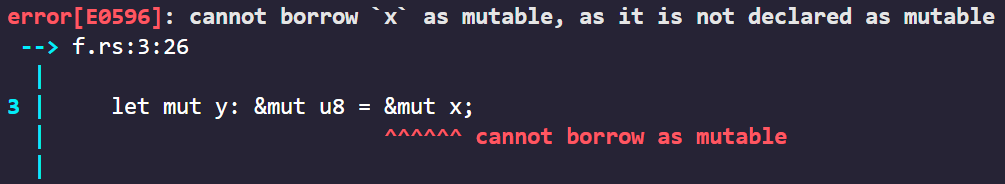
\includegraphics[width=1.0\textwidth]{borrow-mut-from-unmut}
        \caption{Tentativo di \textit{borrow} mutabile di un valore non mutabile}\label{borrow:mut-from-unmut-compile}
    \end{center}
\end{figure}

\noindent Nel Listato~\ref{borrow:two-mutable} si tenta di ottenere due riferimenti mutabili simultaneamente, violando la prima regola di \textit{borrowing}, come riportato nella 
Figura~\ref{borrow:double-mut-compile}.
\begin{figure}[htbp]
    \begin{center}
        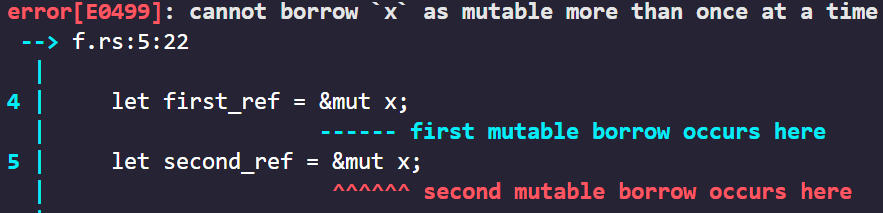
\includegraphics[width=1.0\textwidth]{borrow-double-mut}
        \caption{Tentativo di due \textit{borrow} mutabili allo stesso valore}\label{borrow:double-mut-compile}
    \end{center}
\end{figure}
Il Listato~\ref{borrow:mut-and-unmut} mostra invece il tentativo di ottenere contemporaneamente una reference mutabile e una immutabile, violando la seconda regola di \textit{borrowing}. 
L'errore di compilazione generato è riportato in Figura~\ref{borrow:mut-and-unmut-compile}.
\begin{figure}[htbp]
    \begin{center}
        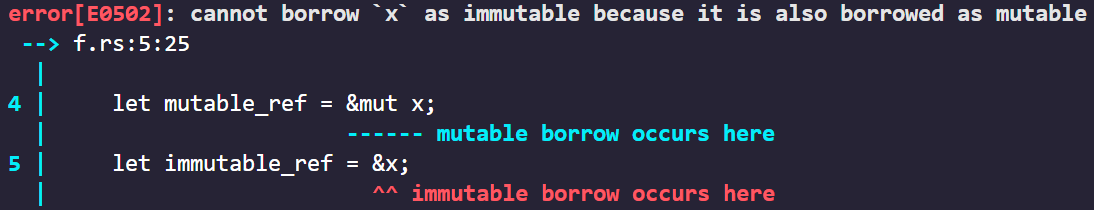
\includegraphics[width=1.0\textwidth]{borrow-mut-and-unmut}
        \caption{Tentativo di \textit{borrow} mutabile e non mutabile simultaneamente allo stesso valore}\label{borrow:mut-and-unmut-compile}
    \end{center}
\end{figure}
Infine, nel Listato~\ref{borrow:dangling-reference} si presenta una \textit{dangling reference}, che viola la terza regola di \textit{borrowing}.
Il risultato è un errore di compilazione, come mostrato in Figura~\ref{borrow:dangling-reference-compile}.
\begin{figure}[htbp]
    \begin{center}
        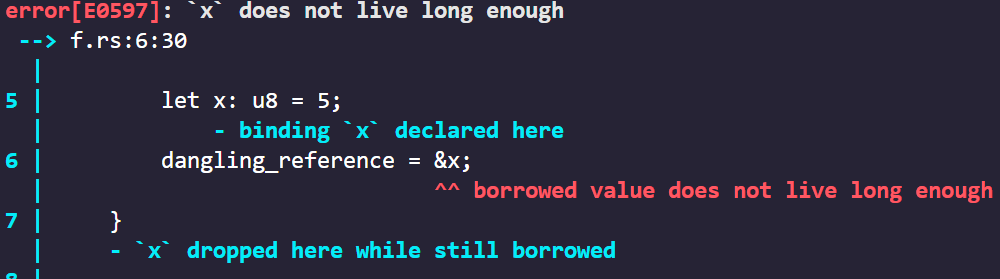
\includegraphics[width=1.0\textwidth]{borrow-dangling-reference}
        \caption{Generazione di un \textit{dangling reference}}\label{borrow:dangling-reference-compile}
    \end{center}
\end{figure}
\vspace{5pt}
Come evidenziato dal Listato~\ref{borrow:dangling-reference}, alcune violazioni delle regole di \textit{borrowing} non riguardano soltanto la mutabilità o il numero di reference presenti, ma coinvolgono anche la durata nel tempo di una reference rispetto al valore referenziato.

Rust gestisce queste relazioni temporali tramite il concetto di \textit{lifetime}, che consente al compilatore di determinare se una reference sarà valida finché necessaria, evitando il rischio di \textit{dangling reference}. \hfill
\vspace{10pt}\\
\noindent Il \textit{Borrow Checker}, quindi, sfrutta anche il sistema delle \textit{lifetime} per garantire che la condivisione dei valori avvenga sempre in modo sicuro e coerente. Questo meccanismo sarà approfondito nella prossima sezione.

\section{Lifetime}
Il sistema delle \textit{lifetime} rappresenta il terzo concetto fondamentale su cui si basa il modello di ownership di Rust. Questo meccanismo viene utilizzato dal \textit{Borrow Checker} per determinare la validità temporale di un prestito (\textit{borrow}).

Nella maggior parte dei casi, le \textit{lifetime} sono implicite e dedotte automaticamente dal compilatore\footnote{Per questo motivo, durante lettura di codice Rust, le annotazioni di \textit{lifetime} sono spesso non visibili.}, in questo caso, vengono definite \textit{lifetime generiche}. In contesti particolari, tuttavia, è necessario esplicitarle, specialmente quando può crearsi ambiguità riguardo la durata di una reference, ad esempio quando si lavora simultaneamente con reference che appartengono a scope differenti.

Si consideri, a riguardo, l'esempio nel Listato~\ref{lifetime:generic-problem}, che mostra come le \textit{lifetime} implicite non siano sufficienti in alcuni contesti:
\begin{lstlisting}[language=Rust, caption={Limitazione delle \textit{lifetime} generiche}, label={lifetime:generic-problem}]
fn biggest(a: &u8, b: &u8) -> &u8 {
    if *a > *b { a } else { b }
}
\end{lstlisting}
Nel Listato~\ref{lifetime:generic-problem} si tenta di restituire un riferimento all'intero più grande tra i due parametri forniti. 
Sebbene il codice possa sembrare corretto, il \textit{Borrow Checker} lo rifiuta, in quanto non può garantire la validità della reference restituita nel tempo.
Il problema nasce dal fatto che le reference \texttt{a} e \texttt{b} potrebbero riferirsi a variabili definite in scope differenti, con durate di vita (\textit{lifetime}) diverse.
Il compilatore, con le \textit{lifetime generiche}, cerca di assegnare la stessa durata ad entrambe le reference, generando ambiguità. \hfill
\vspace{5pt}\\
\noindent Per esplicitare la durata di vita di una reference si utilizza un'annotazione di \textit{lifetime} posta prima del tipo. Questa è rappresentata da un apostrofo seguito da un identificativo; per convenzione si usa una sola lettera, seguento l'ordine alfabetico (\texttt{'a}, \texttt{'b} e così via).
Riferendoci all'esempio del Listato~\ref{lifetime:generic-problem}, la versione corretta viene presentata nel Listato~\ref{lifetime:explicit-solved}, con \textit{lifetime esplicite}:
\begin{lstlisting}[language=Rust, caption={\textit{Lifetime} esplicite}, label={lifetime:explicit-solved}]
fn biggest<'a>(a: &'a u8, b: &'a u8) -> &'a u8 {
    if *a > *b { a } else { b }
}
\end{lstlisting}
Nel Listato~\ref{lifetime:explicit-solved} viene dichiarata una singola \textit{lifetime}, \texttt{'a}, che indica al \textit{Borrow Checker} che i parametri \texttt{a} e \texttt{b} devono avere la stessa durata di vita. Di conseguenza, se le lifetime dei parametri differiscono, la compilazione sarà rifiutata. \hfill
\vspace{10pt}\\
\noindent È importante fare una precisazione: esplicitare una \textit{lifetime} \textbf{non modifica} l'effettiva durata di una variabile. Si tratta solamente di un'indicazione semantica che informa il compilatore dei vincoli temporali che devono essere rispettati tra le \textit{reference} coinvolte. Il \textit{Borrow Checker} utilizza queste annotazioni per verificare la validità dei prestiti nel tempo e può rifiutare il codice se i vincoli non sono coerenti.

A tale scopo, si consideri l'esempio nel Listato~\ref{lifetime:explicit-problem}, che mostra come il \textit{Borrow Checker} possa rifiutare una reference che non rispetti le \textit{lifetime} specificate:
\begin{lstlisting}[language=Rust, caption={Limitazioni delle \textit{lifetime}}, label={lifetime:explicit-problem}]
fn biggest<'a>(a: &'a u8, b: &'a u8) -> &'a u8 {
    if *a > *b { a } else { b }
}

fn main (){
    let result;
    let smaller = 1;
    {
        let bigger = 2;
        result = biggest(&smaller, &bigger);
    }
    println!("Il piu grande e: {}", result);
}
\end{lstlisting}
Nel Listato~\ref{lifetime:explicit-problem}, la funzione \texttt{biggest} viene invocata con due reference che hanno \textit{lifetime} differenti. In particolare, \texttt{bigger} viene definita in uno scope interno, e scade prima che possa essere utilizzata la reference restituita da \texttt{biggest}. Il \textit{Borrow Checker} si accorge di questa incoerenza e segnala un errore di compilazione, come mostrato in Figura~\ref{lifetime:exp-prob-compile}.
\begin{figure}[htbp]
    \begin{center}
        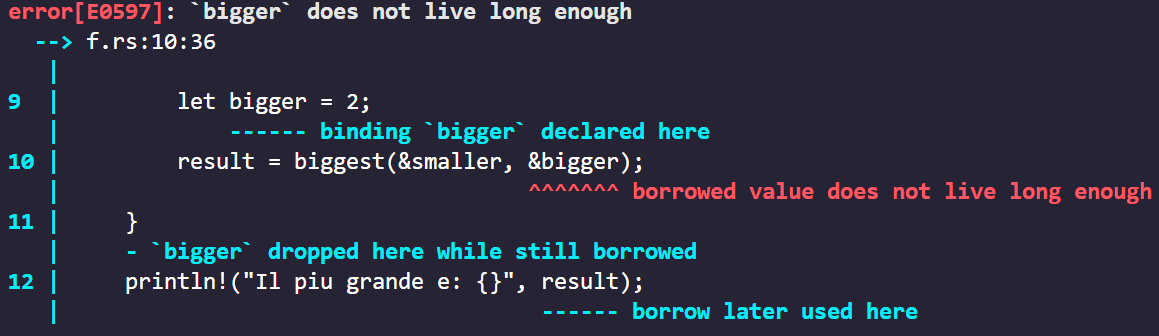
\includegraphics[width=1.0\textwidth]{lifetime-exp-prob}
        \caption{Esempio di violazione delle regole di \textit{Lifetime}}\label{lifetime:exp-prob-compile}
    \end{center}
\end{figure}
\vspace{0pt}\\
\noindent In contesti dove le \textit{lifetime} non vengono esplicitamente annotate, il compilatore applica automaticamente delle regole note come \textit{lifetime elision rules}, che permettono di dedurre in modo implicito i vincoli temporali tra le \textit{reference}. Queste regole sono tre:
\begin{itemize}
    \item A ciascun parametro che è una reference viene assegnata una \textit{lifetime} distinta;
    \item Se c'è una sola reference tra i parametri di ingresso, la sua \textit{lifetime} viene assegnata automaticamente al valore di ritorno (se anch'esso è una reference);
    \item Se ci sono più reference in ingresso, ma una di esse è \texttt{\&self}\footnote{In Rust i metodi delle \texttt{struct} ricevono un parametro implicito, \texttt{self}, che rappresenta l'istanza della struttura sulla quale il metodo è invocato; è un meccanismo analogo a \texttt{self} in Python e a \texttt{this} in Java. Anche \texttt{self} rispetta le regole di \textit{ownership} e \textit{borrowing}: il parametro \texttt{self} trasferisce l'\textit{ownership} dell'istanza, il parametro \texttt{\&self}, invece, indica un riferimento all'istanza (analogamente \texttt{\&mut self} rappresenta un riferimento mutabile).} o \texttt{\&mut self}, allora la \textit{lifetime} di \texttt{self} viene propagata alle eventuali reference in uscita.
\end{itemize}
Infine, esiste una \textit{lifetime} speciale, \texttt{'static}, la quale indica una reference valida per l'intera durata del programma. Questa \textit{lifetime} tipicamente viene utilizzata per dati costanti o risorse allocate a tempo indeterminato.\hfill
\vspace{15pt}\\
\noindent Nel prossimo capitolo verrà mostrato come, grazie a questi concetti, Rust rappresenti un'alternativa valida
per la programmazione di sistema, riuscendo a competere con linguaggi come C e C++.